% !TEX root = ../thesis-example.tex
%
\section{Restructuring the Code}
\label{sec:impr:enzian}

TODO We'll focus on Enzian-Yellow here

\begin{figure}[h]
	\centering
	\captionsetup{justification=centering,margin=2cm}
	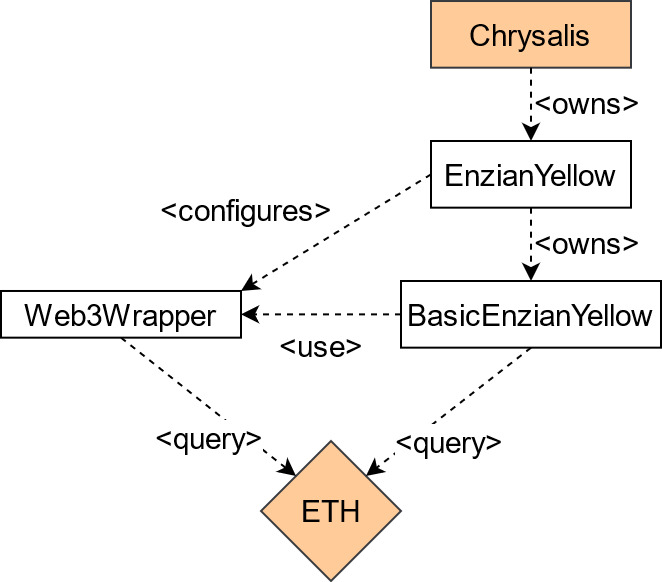
\includegraphics[height=0.5\textwidth]{gfx/system-restructure-enzian-yellow-original}
	\caption{Component structure of the original \emph{Enzian-Yellow} Repository. The components marked in orange are not part of Enzian-Yellow, but interact with it.}
	\label{fig:impr:enzian:original}
\end{figure}

TODO describe the general structure of the original Enzian-Yellow

\subsection{Task Breakdown}

\subsection{Improving the Dependency Hierarchy}

\subsection{Interface for Expansions}

\subsection{Transparency}

\subsection{Minor Improvements}

